\documentclass[reprint,aps,prd,superscriptaddress,showkeys,showpacs]{revtex4-1}
\usepackage{epsfig,amsmath,natbib}

\usepackage{aas_macros}
\usepackage{amssymb}
\usepackage{amsmath}
\usepackage{dsfont}
\usepackage{hyperref}
\usepackage{color}
\usepackage{pbox}
\usepackage{booktabs}
\usepackage[dvipsnames]{xcolor}

\hypersetup{
	colorlinks=false,
	citecolor=green
}

%%%%%%%%%%%%%%%%%
%Custom commands%
%%%%%%%%%%%%%%%%%

\newcommand{\bb}[1]{\mathbf{#1}}
\newcommand{\bbh}[1]{\mathbf{\hat{#1}}}
\newcommand{\h}[1]{\hat{#1}}

\newcommand{\ttt}[1]{\texttt{#1}}

\newcommand\lsim{\mathrel{\rlap{\lower4pt\hbox{\hskip1pt$\sim$}}
        \raise1pt\hbox{$<$}}}
\newcommand\gsim{\mathrel{\rlap{\lower4pt\hbox{\hskip1pt$\sim$}}
        \raise1pt\hbox{$>$}}}

%%%%%%%%%%%%%%%%%%%%%%%%%%%%%%%%%%%%%%%%%%%%%

\begin{document}

\title{Cosmology with Weak Lensing photometric surveys: constraints with redshift tomography of non--Gaussian statistics}

\author{Andrea Petri}
\email{apetri@phys.columbia.edu}
\affiliation{Department of Physics, Columbia University, New York, NY 10027, USA}
\affiliation{Physics Department, Brookhaven National Laboratory, Upton, NY 11973, USA}

\author{Morgan May}
\affiliation{Physics Department, Brookhaven National Laboratory, Upton, NY 11973, USA}

\author{Zolt\'an Haiman}
\affiliation{Department of Astronomy, Columbia University, New York, NY 10027, USA}

\date{\today}

\label{firstpage}

\begin{abstract}
Weak Gravitational Lensing is becoming a popular technique to constrain cosmological parameters, such as the Dark Energy equation of state $w$. When analyzing galaxy surveys, redshift information has proven to be a valuable addition to angular shear correlations. We forecast parameter constraints on the triplet $(\Omega_m,w,\sigma_8)$ for a LSST like galaxy photometric survey, using tomography of the shear-shear power spectrum, convergence peak counts and higher convergence moments. We find that most the cosmological information is contained in the highest redshift galaxies, with redshift tomography further improving the $w$ constraints by only a few $10\%$. We also find that the addition of peak and counts to the power spectrum can significantly improve the constraints on the $(\Omega_m,w)$ doublet. We evaluate the effect of uncorrected photometric redshift systematics on parameter constraints. We find that different statistics lead to different bias directions in parameter space, leaving a window open for self--calibration. 
\end{abstract}


\keywords{Weak Gravitational Lensing --- Simulations --- Systematic effects: photometry --- Methods: numerical, statistical}
\pacs{98.80.-k, 95.36.+x, 95.30.Sf, 98.62.Sb}

\maketitle


%%%%%%%%%%%%%%%%%%%%%%%%%% INTRO %%%%%%%%%%%%%%%%%%%%%%%%%%%%%%%%%%%%%%%%%%%%%%%%%%%%%%%%

\section{Introduction}
%
Weak Gravitational Lensing is a promising technique to probe the Large Scale Structure of the universe in which the tracers are unbiased \citep{wlreview}. This technique has the potential of improving significantly the constraints on the Dark Energy equation of state $w$ because it is most sensitive to the matter density fluctuations at the non--linear stage. Cosmology inferences from Weak Lensing observations have been produced for past (CFHTLenS \citep{cfht1}) and current (DES \citep{DES}) surveys, and are being planned for future experiments as well (LSST \citep{LSST}, WFIRST \citep{WFIRST}, Euclid \citep{Euclid}). Because of the non-linear nature of the density fluctuations probed by Weak Lensing, cosmological information might leak from quadratic statistics (such as two point functions and power spectra) into more complicated non-Gaussian statistics, for which forward modeling from cosmological parameters requires numerical simulations of cosmic shear fields. Different examples of these non-Gaussian statistics, and their cosmological information content, have been investigated extensively in the literature (see \citep{MinkJan,PeaksJan,NG-Marian,NG-Jain1,NG-Jain2,NG-Jain3,NG-Refregier,NG-Dietrich} for a non comprehensive list). The constraining power of Weak Lensing power spectra with the addition of redshift tomography information have been extensively investigated in the literature (see \citep{SongKnox,FangHaiman07,Huterer2006}). In this work we concentrate on the constraining power of a subset of these non-Gaussian statistics combined with redshift tomography in a LSST-like survey. Previous work on redshift tomography with Weak Lensing Minkowski functionals is also present in the literature \citep{MinkJan}. We also investigate the effects of uncorrected photometric redshift systematics on parameter constraints when using redshift tomography. This work is organized as follows: we give an outline of the shear simulations we use in this work, followed by descriptions of the convergence reconstruction procedure and forward modeling of galaxy shape and photometric redshift systematics. We then give an overview of the parameter inferences techniques we used to forecast constraints on cosmology. We then discuss the main results of this work and present our conclusions as well as prospects for future work.  

%%%%%%%%%%%%%%%%%%%%%%%%%% METHODS %%%%%%%%%%%%%%%%%%%%%%%%%%%%%%%%%%%%%%%%%%%%%%%%%%%%%%

\section{Methods}

%%%%%%%%

\subsection{Cosmic shear simulations}
\label{sec:shearsim}
We review the procedure used for generating mock shear catalogs. We consider a fiducial flat $\Lambda$CDM universe with $(h,\Omega_m,\Omega_\Lambda,\Omega_b,w,\sigma_8,n_s)=(0.72,0.26,0.74,0.046,-1,0.8,0.96)$. We examine different variations of the $\bb{p}=(\Omega_m,w,\sigma_8)$ triplet and run one $N$--body simulation for each choice of $\bb{p}$, using the public code \ttt{Gadget2} \citep{Gadget2}. The simulations have a comoving box size of $L_b=260\,{\rm Mpc}/h$ and contain $512^3$ dark matter particles, which correspond to a mass resolution of $M_p\approx 10^{10}M_{\rm sun}$ per particle. The three dimensional outputs of the $N$--body simulations are sliced in sequences of two dimensional lenses $120 \,{\rm Mpc}$ thick, which are lined up perpendicular to the line of sight between the observer on Earth and a source at redshift $z_s$. We make use of the multi--lens--plane algorithm \citep{RayTracingJain,RayTracingHartlap} to trace the deflections of light rays originating at $z=0$ through the system of lenses until $z$. To accomplish this task, we make use of the \ttt{LensTools} \citep{LensTools-ASCL,LensTools-paper} implementation of the multi--lens--plane algorithm. An observed galaxy position $\pmb{\theta}$ on the sky today corresponds to a real galaxy angular position $\pmb{\beta}(\pmb{\theta},z_s)$, which can be calculated using the \ttt{LensTools} pipeline by solving the lensing ODE up to redshift $z_s$. The Jacobian of $\pmb{\beta}(\pmb{\theta},z_s)$ is a $2\times 2$ matrix that contains information about the cosmic shear field at $\pmb{\theta}$ integrated along the line of sight. 
%
\begin{equation}
\label{meth:sheareqn}
\frac{\partial\beta_i(\pmb{\theta},z_s)}{\partial \theta_j} = 
\begin{pmatrix}
1-\kappa(\pmb{\theta})-\gamma^1(\pmb{\theta}) & -\gamma^2(\pmb{\theta}) \\
-\gamma^2(\pmb{\theta}) & 1-\kappa(\pmb{\theta})+\gamma^1(\pmb{\theta})\\
\end{pmatrix}
\end{equation}  
%
The quantities that appear in equation (\ref{meth:sheareqn}) are the convergence $\kappa$, which is the source magnification due to lensing, and the cosmic shear $\pmb{\gamma}$, which is a measurement of the source ellipticity due to lensing from Large Scale Structure, assuming the non lensed shape is a circle. 
We simulate $N_g = 10^6$ random galaxy positions $\{\pmb{\theta}_g\}$ distributed uniformly in a field of view of size $\theta_{\rm FOV}^2=(3.5{\rm deg})^2$, which correspond to a galaxy angular density of $n_g=22\,\rm{arcmin}^{-2}$. The galaxies have a distribution in redshift which mimics the one expected in the LSST survey
\begin{equation}
\label{meth:galdistr}
n(z) = n_0\left(\frac{z}{z_0}\right)^2\exp\left(-\frac{z}{z_0}\right)
\end{equation}  
%
with $z_0=0.3$ and $n_0$ a normalization constant fixed so that $n(z)$ integrates to the total number of galaxies $N_g$. The galaxies have a maximum redshift $z_{\rm max}=3$. For each galaxy we compute the cosmic shear at $\pmb{\theta}_g$ using equation (\ref{meth:sheareqn}), producing a shear catalog $\{\pmb{\gamma}_g\}$. Different random realizations of a shear catalog $\{\pmb{\gamma}_g\}_r$ can be obtained rotating and periodically shifting the Large Scale Structure in the $N$--body snapshots according to the procedure explained in \citep{PetriVariance}. We produce $N_r=16000$ pseudo--independent realizations of the shear catalog $\{\pmb{\gamma}_g\}$. These shear realization cover the total survey area of LSST 10 times.
We repeat the above procedure for $P=100$ different combinations of the parameter triplet $\bb{p}$, sampled according to a Latin hypercube scheme. The sampling procedure is the same described in \citep{CFHTMink,CFHTPeaks}. The parameter space sampling we adopted for our simulations is shown in Figure \ref{fig:simdesign}

\begin{figure*}
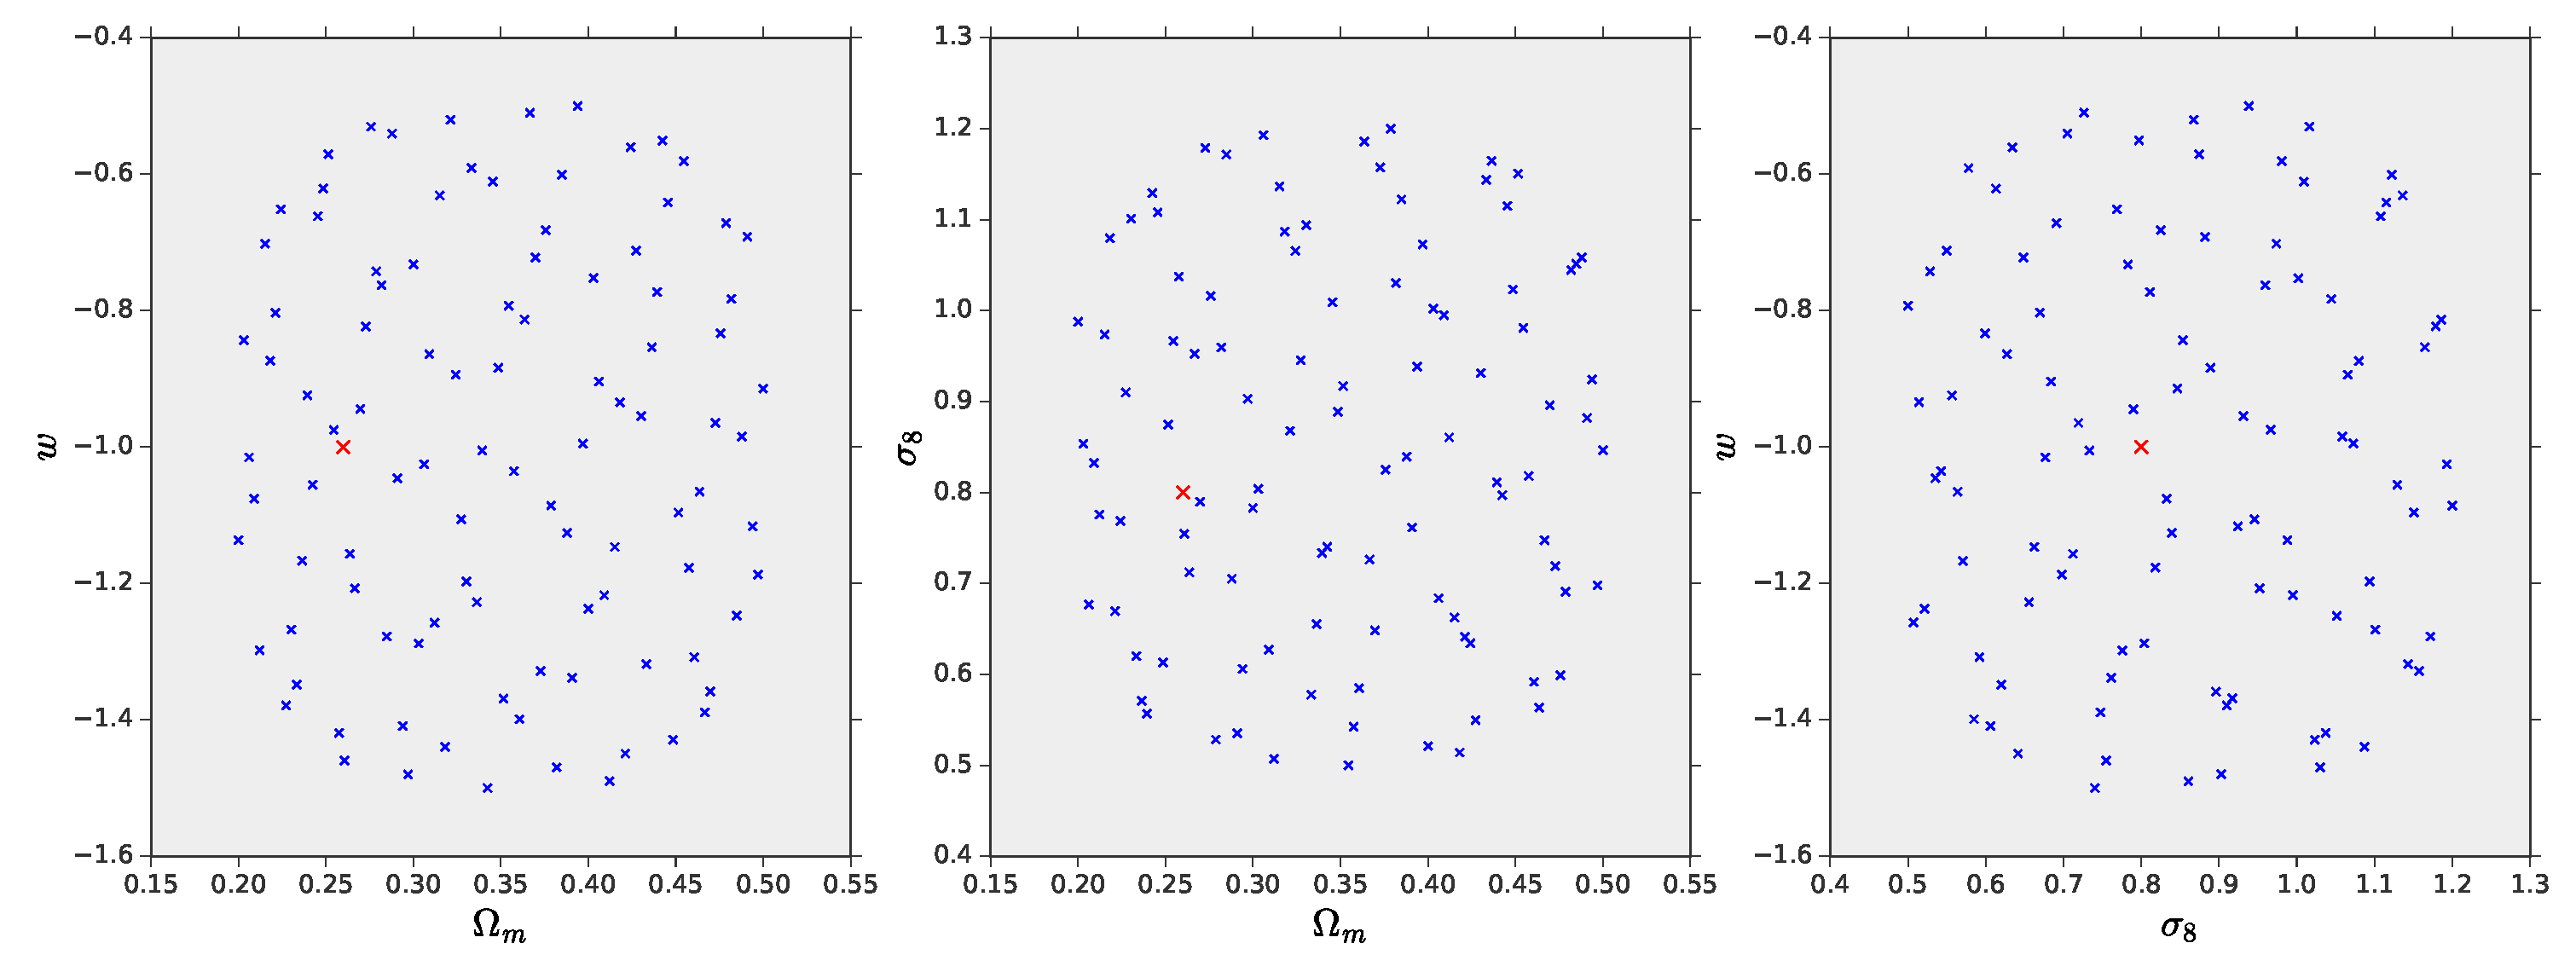
\includegraphics[scale=0.35]{Figures/design.eps}
\caption{Parameter space sampling chosen for our simulations. We show both the sampling in the $(\Omega_m,w)$ (left), $(\Omega_m,\sigma_8)$ (center) and $(\sigma_8,w)$ (right) slices of the parameter space. The fiducial cosmology has been marked in red.}
\label{fig:simdesign}
\end{figure*}
%
For each of the parameter choices in Figure \ref{fig:simdesign}, the $N$--body initial conditions are generated using the same random seed. In addition to these simulations, we produce simulated shear catalogs for a fiducial $\Lambda$CDM universe with $\bb{p}_0=(0.26,-1,0.8)$. In this case the randomization procedure is based on 5 independent $N$--body simulations, and the same number $N_r=16000$ of pseudo--independent catalog realizations is produced. This additional simulation set serves two purposes: it provides an independent dataset from which to measure covariance matrices and it provides a way to construct mock observations that are independent on the simulations on which the cosmological forward model is trained. For the fiducial dataset we chose to base the shear randomization procedure on 5 independent $N$--body simulations to ensure the independence of the $N_r$ realizations for the purpose of estimating covariance matrices. \citep{PetriVariance} recently showed that, even with only one $N$--body simulation a few $10^4$ independent realizations can be produced.   

%%%%%%%%

\subsection{Forward modeling of systematics}
We give an overview of the shear systematics included in this work. 

The measured galaxy ellipticity $\pmb{\epsilon}$ is an estimate of the cosmic shear $\pmb{\gamma}$ due to Large Scale Structure if the non--lensed galaxy shape is a circle. If this assumption is relaxed, the measured galaxy ellipticity $\pmb{\epsilon}_{\rm m}$ can be modeled as a cosmic shear term plus a noise term \citep{wlreview}
\begin{equation}
\pmb{\epsilon}_{\rm m} = \pmb{\gamma} + \pmb{\epsilon}_{\rm n}
\end{equation} 
%
where $\pmb{\epsilon}_{\rm n}$ is a random Gaussian variable with zero mean and redshift dependent variance $\sigma_n(z_s)=0.15+0.035z_s$. This is equivalent to say that the cosmic shear inferred from ellipticity observations $\pmb{\gamma}_{\rm m}$ can be written as the sum of the true cosmic shear plus a noise term $\pmb{\gamma}_{\rm n}$ with the same statistical properties as $\pmb{\epsilon}_{\rm n}$. 
We add independent random realizations of the shape noise $\pmb{\gamma}_{\rm n}$ to each of the $N_r$ shear catalogs. Each shape noise realization is generated with a different random seed. The same random seeds are used to generate shape noise catalogs across simulations with different cosmological parameters $\{\bb{p}_i\}$.

In addition to shape noise contributions to the observed galaxy ellipticity we consider photometric redshift errors as an additional contamination source in the simulated catalogs. In photometric surveys such as LSST, the source redshift $z_s$ is estimated measuring the source luminosity in a finite small set of optical frequency bands. Using this compressed luminosity information rather than the full spectrum introduces biases in redshift estimation. Forward modeling of the cosmic shear using the procedure described in \S~\ref{sec:shearsim}, as well as the shape noise contributions, assume a correct redshift distributions $n(z)$. An incorrect binning of observed galaxy redshifts according to the measured photometric distribution $n_p(z_p)$ can propagate the redshift measurement errors all the way to cosmological parameter constraints if the latter take advantage of redshift tomography. One of the goals of this work is to evaluate the size of this effect, assuming photometric redshift errors (photo-$z$) are left uncorrected. 

We model effect of photo-$z$ errors as a constant bias term $b_{\rm ph}(z_s)$ plus a random Gaussian component with variance $\sigma_{\rm ph}(z_s)$
\begin{equation}
\label{meth:photoz-correction}
z_p(z_s) = z_s + b_{\rm ph}(z_s) + \sigma_{\rm ph}(z_s)\mathcal{N}(0,1)   
\end{equation}
%
where $\mathcal{N}(0,1)$ is the standard normal distribution. We bin the $N_g$ galaxies in our simulated catalogs in 5 redshift bins $\bar{z}_b$, $b=1...5$. Several models have been proposed in the literature for the photometric bias $b_{\rm ph}(z_s)$ (see for example \citep{Huterer2006}) and variance $\sigma_{\rm ph}(z_s)$ (see for example \citep{LSSTSciBook}). We chose the photo-$z$ bias and variance functions in equation (\ref{meth:photoz-correction}) to be the science requirements contained in the LSST Science Book \citep{LSSTSciBook}, namely $b(z_s)=0.003(1+z_s)$ and $\sigma(z_s)=0.02(1+z_s)$. 

\begin{figure}
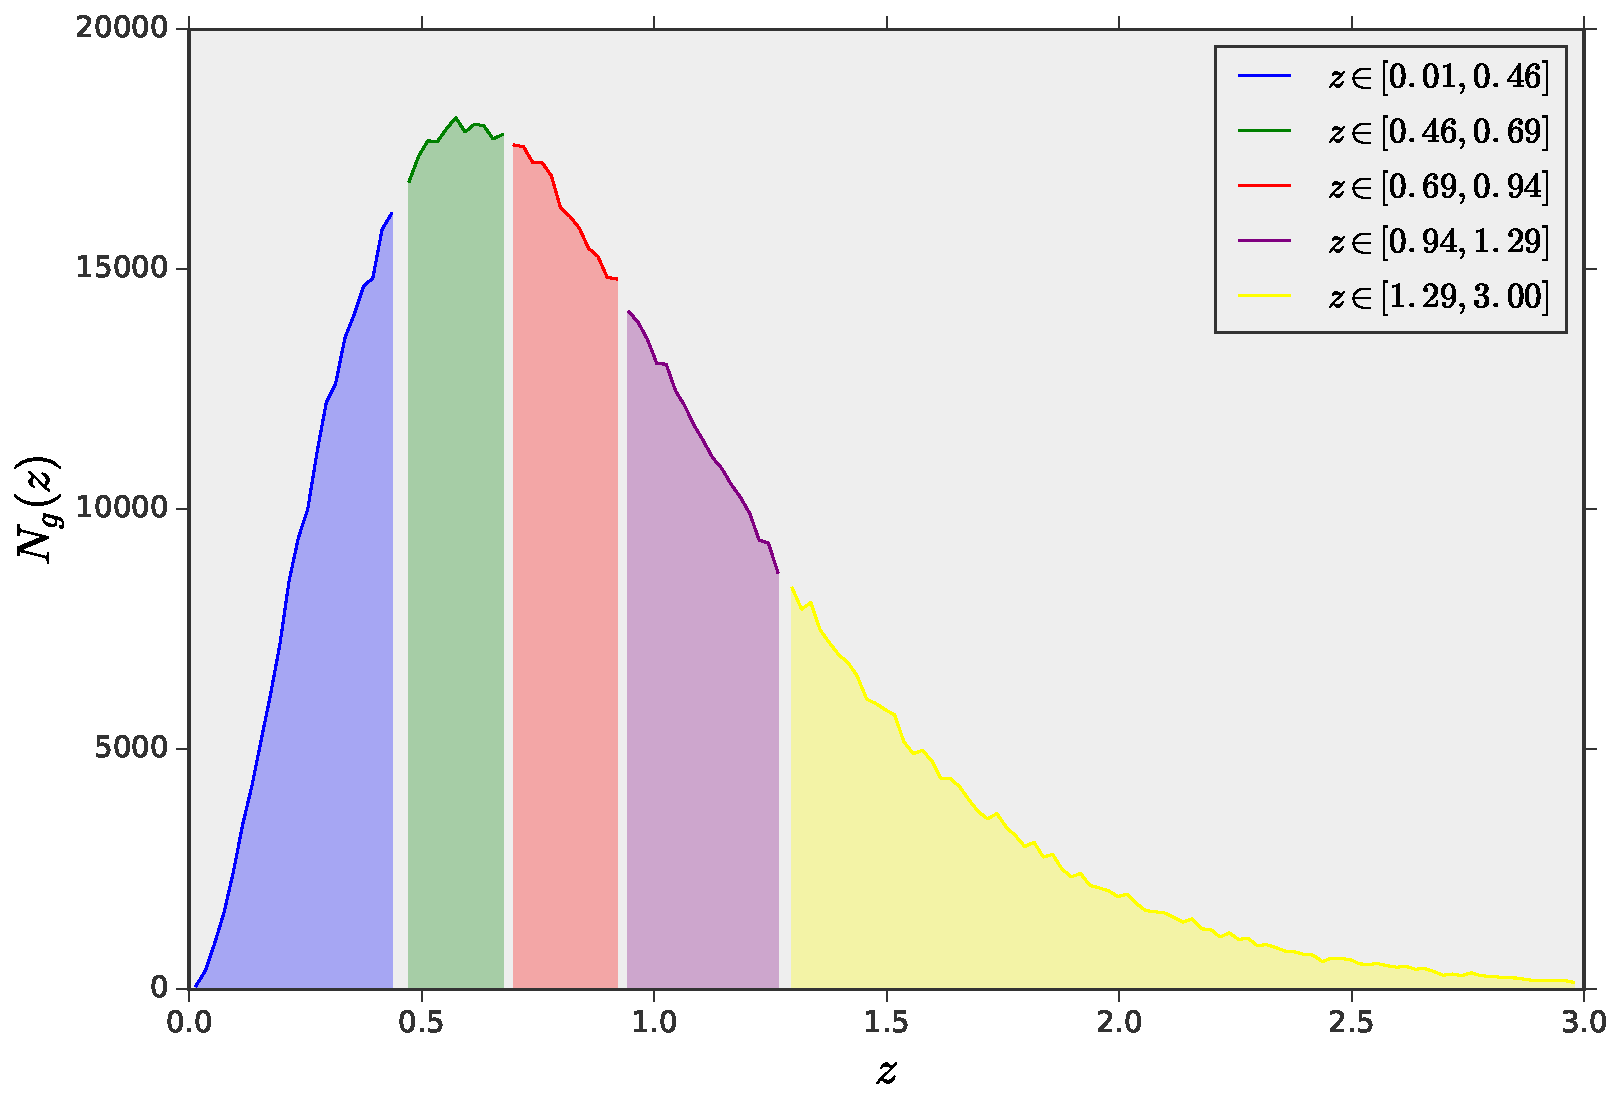
\includegraphics[scale=0.3]{Figures/galdistr.pdf}
\caption{Galaxy distribution assumed throughout this work (see equation (\ref{meth:galdistr})), along with the choice of the redshift bins $\bar{z}_b$. Our galaxy sample consists of $N_g=10^6$ galaxies. The figure shows the number of galaxies $N_g(z)$ at each redshift $z$.}
\label{fig:galdistr}
\end{figure}

We generate mock observations by applying an independent random realization of the photo-$z$ correction (\ref{meth:photoz-correction}) to each catalog realization in the fiducial cosmology $\bb{p}_0$ and by re--binning the galaxies according to their photometric redshifts $z_p$. In the remainder of the paper we use the following notation: we indicate a shear realization $r$ in cosmology $\bb{p}$ with shape noise added as $\h{\pmb{\gamma}}_r(\pmb{\theta}_g,z_g;\bb{p})$, and we indicate a mock observation as $\h{\pmb{\gamma}}_{\rm obs}(\pmb{\theta}_g,z_g)$.           

%%%%%%%%

\subsection{Convergence reconstruction}
In this paragraph we describe the procedure we used to construct convergence maps $\kappa$ from the simulated shear catalogs $\pmb{\gamma}$. We consider a two dimensional square pixel grid of area $\theta_{\rm FOV}^2$ and with 512 pixel per side. This correspond to a linear pixel resolution of $0.5 \rm{arcmin}$. We assign a shear value $\pmb{\gamma}(\pmb{\theta}_p,\bar{z}_b)$ to each pixel $\pmb{\theta}_p$ according to the following procedure
\begin{equation}
\pmb{\gamma}(\pmb{\theta}_p,\bar{z}_b) = \frac{\sum_{g=1}^{N_g}\pmb{\gamma}(\pmb{\theta}_g,z_g)W(\pmb{\theta}_g,\pmb{\theta}_p;z_g,\bar{z}_b)}{\sum_{g=1}^{N_g}W(\pmb{\theta}_g,\pmb{\theta}_p;z_g,\bar{z}_b)}
\end{equation}   
%
We chose a top--hat window function
\begin{equation}
W(\pmb{\theta}_g,\pmb{\theta}_p;z_g,\bar{z}_b) = 
\begin{cases}
1 \,\,\,\,{\rm if}\,\,\,\, \pmb{\theta}_g\in\pmb{\theta}_p,z_g\in\bar{z}_b \\
0 \,\,\,\,{\rm otherwise}
\end{cases}
\end{equation} 
%
The convergence $\kappa(\pmb{\theta}_p)$ can be reconstructed from the $E$--mode of the shear field, which is evaluated from the Fourier Transform of the pixelized shear $\pmb{\gamma}(\pmb{\theta}_p,\bar{z}_b)$
\begin{equation}
\label{meth:psdefinition}
\tilde\kappa(\pmb{\ell},\bar{z}_b) = \left(\frac{\tilde{\gamma}^1(\pmb{\ell},\bar{z}_b)(\ell_x^2-\ell_y^2)+2\ell_x\ell_y\tilde{\gamma}^2(\pmb{\ell},\bar{z}_b)}{\ell_x^2+\ell_y^2}\right) e^{-\frac{\ell^2\theta_G^2}{2}}
\end{equation}
%
We chose the Gaussian filter smoothing scale $\theta_G=0.5\,{\rm arcmin}$ to correspond to the linear pixel resolution. Inverting the Fourier Transform yields the pixelized map $\kappa(\pmb{\theta}_p,\bar{z}_b)$. We apply this procedure to both the shear realizations $\h{\pmb{\gamma}}_r(\pmb{\theta}_g,z_g;\bb{p})$ and the mock observations $\h{\pmb{\gamma}}_{\rm obs}(\pmb{\theta}_g,z_g)$, yielding convergence realizations $\h{\kappa}_r(\pmb{\theta}_p,\bar{z}_b;\bb{p})$ and mock convergence observations $\h{\kappa}_{\rm obs}(\pmb{\theta}_p,\bar{z}_b)$. 

We measure a variety of summary statistics from the pixelized convergence maps, which will then be used to forecast parameter constraints and biases. We consider three kinds of summary statistics, namely the $\kappa$ tomographic power spectrum $P^{\kappa\kappa}(\ell,\bar{z}_b,\bar{z}_{b'})$, the tomographic peak counts $n_{\rm pk}(\nu,\bar{z}_b)$ and a set of $\kappa$ moments $\pmb{\mu}(\bar{z}_b)$. The tomographic power spectrum is defined as 
\begin{equation}
\langle\tilde{\kappa}(\pmb{\ell},\bar{z}_b)\tilde{\kappa}(\pmb{\ell}',\bar{z}_{b'})\rangle = (2\pi)^2\delta_D(\pmb{\ell}+\pmb{\ell}')P^{\kappa\kappa}(\ell,\bar{z}_b,\bar{z}_{b'})
\end{equation}
%
Because the $\kappa$ field is statistically isotropical, the expectation value $\langle\rangle$, for each realization $r$, is taken over all the modes $\pmb{\ell}$ which have the same magnitude $\ell=\vert\pmb{\ell}\vert$. The peak count statistic $n_{\rm pk}(\nu,\bar{z}_b)$ is defined as the number of the $\kappa$ local maxima of a certain height $\kappa_{\rm max}=\nu\sigma_0$, where $\sigma_0$ is the $\kappa$ standard deviation over pixels. The $\kappa$ moments $\pmb{\mu}(\bar{z}_b)$ are defined as follows (see \citep{Matsubara10,Munshi12,MinkPetri}) 
%
\begin{equation}
\label{meth:momdef}
\begin{matrix}
\pmb{\mu} = (\pmb{\mu}_2,\pmb{\mu}_3,\pmb{\mu}_4) \\ \\
\pmb{\mu}_2 = (\langle\kappa^2\rangle,\langle\vert\nabla\kappa\vert^2\rangle) \\ \\
\pmb{\mu}_3 = (\langle\kappa^3\rangle,\langle\kappa\vert\nabla\kappa\vert^2\rangle,\langle\kappa^2\nabla^2\kappa\rangle) \\ \\
\pmb{\mu}_4 = (\langle\kappa^4\rangle_c,\langle\kappa^2\vert\nabla\kappa\vert^2\rangle_c,\langle\kappa^3\nabla^2\kappa\rangle_c,\langle\vert\nabla\kappa\vert^4\rangle_c)
\end{matrix}
\end{equation}
%
In equation (\ref{meth:momdef}) the gradients $\nabla$ are evaluated using finite differences between $\kappa$ values at neighboring pixels and the expectation values $\langle\rangle$ for each realization $r$ are taken over the $512^2$ pixels in the map. The subscript $c$ indicates that we consider only the connected parts of the quartic $\kappa$ moments. In the definition of the peak counts and convergence moments we omitted the redshift index $\bar{z}_b$ for notational simplicity. In the next paragraph we describe the statistical methods we use to infer cosmological parameter estimates $\bbh{p}$ from mock observations $\h{\kappa}_{\rm obs}(\pmb{\theta}_p,\bar{z}_b)$ using the summary statistics $P^{\kappa\kappa}(\ell,\bar{z}_b,\bar{z}_{b'})$, $n_{\rm pk}(\nu,\bar{z}_b)$, $\pmb{\mu}(\bar{z}_b)$.   

%%%%%%%%

\subsection{Parameter inference}
We adopt a Bayesian framework to forecast parameter constraints. We indicate as $\bb{d}$ a summary statistic vector (which can be any of $P^{\kappa\kappa},n_{\rm pk},\pmb{\mu}$ or a combination of the former). We label $\bb{d}(\bb{p})$ the sample mean of $\bb{d}$ over the $N_r=16000$ simulated realizations in cosmology $\bb{p}$ and we label $\bbh{d}_r$ the summary statistic measured in realization $r$ of the fiducial cosmology $\bb{p}_0$. Both $\bb{d}(\bb{p}),\bbh{d}_r$ are measured taking galaxy shape noise into account. We further label $\bbh{d}_{\rm obs}$ the summary statistic measured in a mock observation in which $\kappa$ has been measured taking photo-$z$ errors into account. $\bbh{d}_{\rm obs}$ is measured averaging a random sample of $N_{\rm FOV}=1600$ realizations of the fiducial cosmology with photo-$z$ errors added. This number has been chosen to mimic the survey are of LSST $\Omega_{\rm LSST}=N_{\rm FOV}\theta_{\rm FOV}^2$. Assuming no prior knowledge of the parameters $\bb{p}$, we can write the parameter likelihood $\mathcal{L}$ given the observation $\bbh{d}_{\rm obs}$ using the Bayes theorem
%
\begin{equation}
\label{meth:paramlikelihood}
-2\log\mathcal{L}(\bb{p}\vert \bbh{d}_{\rm obs}) = (\bbh{d}_{\rm obs} - \bb{d}(\bb{p}))^T\bb{C}^{-1}(\bbh{d}_{\rm obs} - \bb{d}(\bb{p}))
\end{equation}  
%
The parameter likelihood (\ref{meth:paramlikelihood}) can be evaluated at every point $\bb{p}$ in parameter space by interpolating $\bb{d}(\bb{p})$ between simulation points $\{\bb{p}_i\}$ using a Radial Basis Function (RBF) interpolation (see \citep{CFHTMink,LensTools-paper}). $\bb{C}$ is the $\bb{d}$ covariance matrix and is assumed to be $\bb{p}$--independent. In practice we replace $\bb{C}$ with its estimated value $\bbh{C}$ from $N_r=16000$ realizations of the summary statistics $\bbh{d}_r$ in the fiducial cosmology $\bb{p}_0$ without photo-$z$ errors
%
\begin{equation}
\bbh{d}_{\rm mean} = \frac{1}{N_r}\sum_{r=1}^{N_r}\bbh{d}_r 
\end{equation}
%
\begin{equation}
\bbh{C} = \frac{1}{N_r-1}\sum_{r=1}^{N_r} (\bbh{d}_r-\bbh{d}_{\rm mean})(\bbh{d}_r-\bbh{d}_{\rm mean})^T
\end{equation} 
%
Cosmological parameter values $\bbh{p}$ can be inferred from equation (\ref{meth:paramlikelihood}) by looking at the location at which the likelihood $\mathcal{L}(\bb{p}\vert\bbh{d}_{\rm obs})$ is maximum. Parameter errors $\Delta\bbh{p}$ can be inferred from the likelihood confidence contours. Approximate estimates of $\bbh{p},\Delta \bbh{p}$ can be obtained approximating the model statistic $\bb{d}(\bb{p})$ dependency on parameters as linear in $\bb{p}$ provided $\bb{p}$ is not too far from the fiducial model $\bb{p}_0$
\begin{equation}
\label{meth:linapprox}
\bb{d}(\bb{p}) = \bb{d}(\bb{p}_0) + \bb{M}(\bb{p}-\bb{p}_0) + O(\vert\bb{p}-\bb{p}_0\vert^2)
\end{equation} 
%
Where we defined $(\bb{M})_{i\alpha}=(\partial d_i(\bb{p})/\partial p_\alpha)_{\bb{p}_0}$ as the statistic first derivative with respect to cosmology. We evaluate $\bb{M}$ with finite differences on the smooth RBF interpolation of the summary statistic $\bb{d}(\bb{p})$. This linear approximation allows for a fast estimate of $\bbh{p}$ in terms of $\bbh{d}_{\rm obs}$
\begin{equation}
\label{meth:parestimate}
\bbh{p} = \bb{p}_0 + (\bb{M}^T\bbh{\Psi}\bb{M})^{-1}\bb{M}^T\bbh{\Psi}(\bbh{d}_{\rm obs}-\bb{d}(\bb{p}_0))
\end{equation}
%
Here we indicated $\bbh{\Psi}=\bbh{C}^{-1}$ as the summary statistic precision matrix. With the linear approximation (\ref{meth:linapprox}) the parameter likelihood (\ref{meth:paramlikelihood}) is a multivariate Gaussian in $\bb{p}$ and its width $\bbh{\Sigma}$ can be estimated as 
\begin{equation}
\label{meth:parcovestimator}
(\bbh{\Sigma})_{\alpha\beta} = -\left(\frac{\partial^2 \log \mathcal{L}(\bb{p})}{\partial p_\alpha \partial p_\beta}\right)^{-1}_{\bb{p}_0} = ((\bb{M}^T\bbh{\Psi}\bb{M})^{-1})_{\alpha\beta}
\end{equation}
%
The $1\sigma$ square parameter errors $\Delta \bbh{p}^2$ are the diagonal entries of $\bbh{\Sigma}$. The parameter covariance estimator (\ref{meth:parcovestimator}) is the same that one gets adopting a Fisher Matrix formalism for parameter forecasts (see \citep{astroMLText} for a possible reference).

When the dimension $N_b$ of the summary statistics space is large, numerical issues can arise in the estimation of the parameter error bars if the covariance matrix $\bbh{C}$ is measured from simulations. When $N_r$ independent realizations are used to estimate $\bbh{C}$, its inverse $\bbh{\Psi}$ is biased by a constant factor (see \citep{Hartlap07,Taylor12,Taylor14}) that can be taken into account. When the bias correction is applied, we can calculate the expectation value of the covariance estimator (\ref{meth:parcovestimator}) (see again\citep{Taylor14})
\begin{equation}
\label{meth:covdegradation}
\langle\bbh{\Sigma}\rangle = \left(\frac{N_r-N_b+N_p-1}{N_r-N_b-2}\right)\bb{\Sigma}
\end{equation}   
%
where $\bb{\Sigma}$ is the asymptotic covariance one obtains with an infinite number of realizations and $N_p$ is the number of parameters we are estimating, in this case 3. The scatter of the parameter estimates (\ref{meth:parestimate}) on the other hand scales as 
\begin{equation}
\label{meth:estdegradation}
\langle{\rm Cov}(\bbh{p})\rangle = \left(\frac{N_r-2}{N_r-N_b+N_p-2}\right)\bb{\Sigma}
\end{equation}
%
Although equations (\ref{meth:covdegradation}) and (\ref{meth:estdegradation}) agree in the limit $N_r\rightarrow\infty$, they can be different when a finite number of realizations is used. More in detail, the degradation factor in the parameter covariance estimate in (\ref{meth:covdegradation}) is of order $1+(1+N_p)/N_r$, while the actual scatter of the estimates $\bbh{p}$ is of order $1+(N_b-N_p)/N_r$. These numbers can very different if $N_b$ is big. This means that the parameter error bar estimate (\ref{meth:covdegradation}) is too conservative if $N_b/N_r$ is of order unity. This could be likely the case in the analysis we are carrying because of the inclusion of tomography information. In order to avoid these error degradation issues, we apply dimensional reduction techniques to the summary statistics we are considering. These techniques are explained in the next paragraph.   


%%%%%%%%

\subsection{Dimensionality reduction}
We apply Principal Component Analysis techniques (see \citep{astroMLText} for example) to reduce the dimensionality of our summary statistics while preserving the cosmological information content. Consider the model statistic $\bb{d}(\bb{p})$, and think of it in terms of a $P\times N_b$ matrix $d_{pi}$. Consider the whitened model matrix
\begin{equation}
\Delta_{pi} = P\frac{d_{pi}}{\sum_{q=1}^Pd_{qi}} - 1
\end{equation} 
%
We perform a Singular Value Decomposition (SVD) of $\Delta$ 
\begin{equation}
\bb\Delta = \bb{L}\bb{\Lambda} \bb{R}
\end{equation}
%
where $L$ is $P\times Q$, $\bb{\Lambda}={\rm diag}(\Lambda_1,...,\Lambda_Q)$ and $\bb{R}$ is $Q\times N_b$ and $Q={\min}(P,N_b)$. $R_{ni}$ is the $i$-th component of the $n$-th basis vector in statistics space. The singular value $\Lambda_n$ is the variance of the whitened summary statistic along the $n$-th basis vector. We assume that only summary statistic projections on the first $N_c$ basis vectors contain relevant cosmological information, and $N_c<N_b$ is a number that has to be determined from the simulations. Let $\bb{R}(N_c)$ be a matrix made of the first $N_c$ rows of $\bb{R}$ (we assume that the singular values $\Lambda_i$ are sorted). We define the PCA projection of a summary statistic $\bbh{d}$ on $N_c$ principal components as 
\begin{equation}
\label{meth:pcaprojection}
\h{d}_n(N_c) = \sum_{i=1}^{N_b}(\bb{R}(N_c))_{ni}\left(P\frac{\h{d}_i}{\sum_{p=1}^P d_{pi}}-1\right) 
\end{equation} 
%
In this way we hope to capture the cosmological information contained in $\bbh{d}$ by projecting it on the $N_c<N_b$ principal components that vary the most with cosmology parameters. In the next section we outline the main results of this work.  
%%%%%%%%%%%%%%%%%%%%%%% RESULTS %%%%%%%%%%%%%%%%%%%%%%%%%%%%%%%%%%%%%%%%%%%%%%%%%%%%%%%%%

\section{Results}

\begin{figure*}
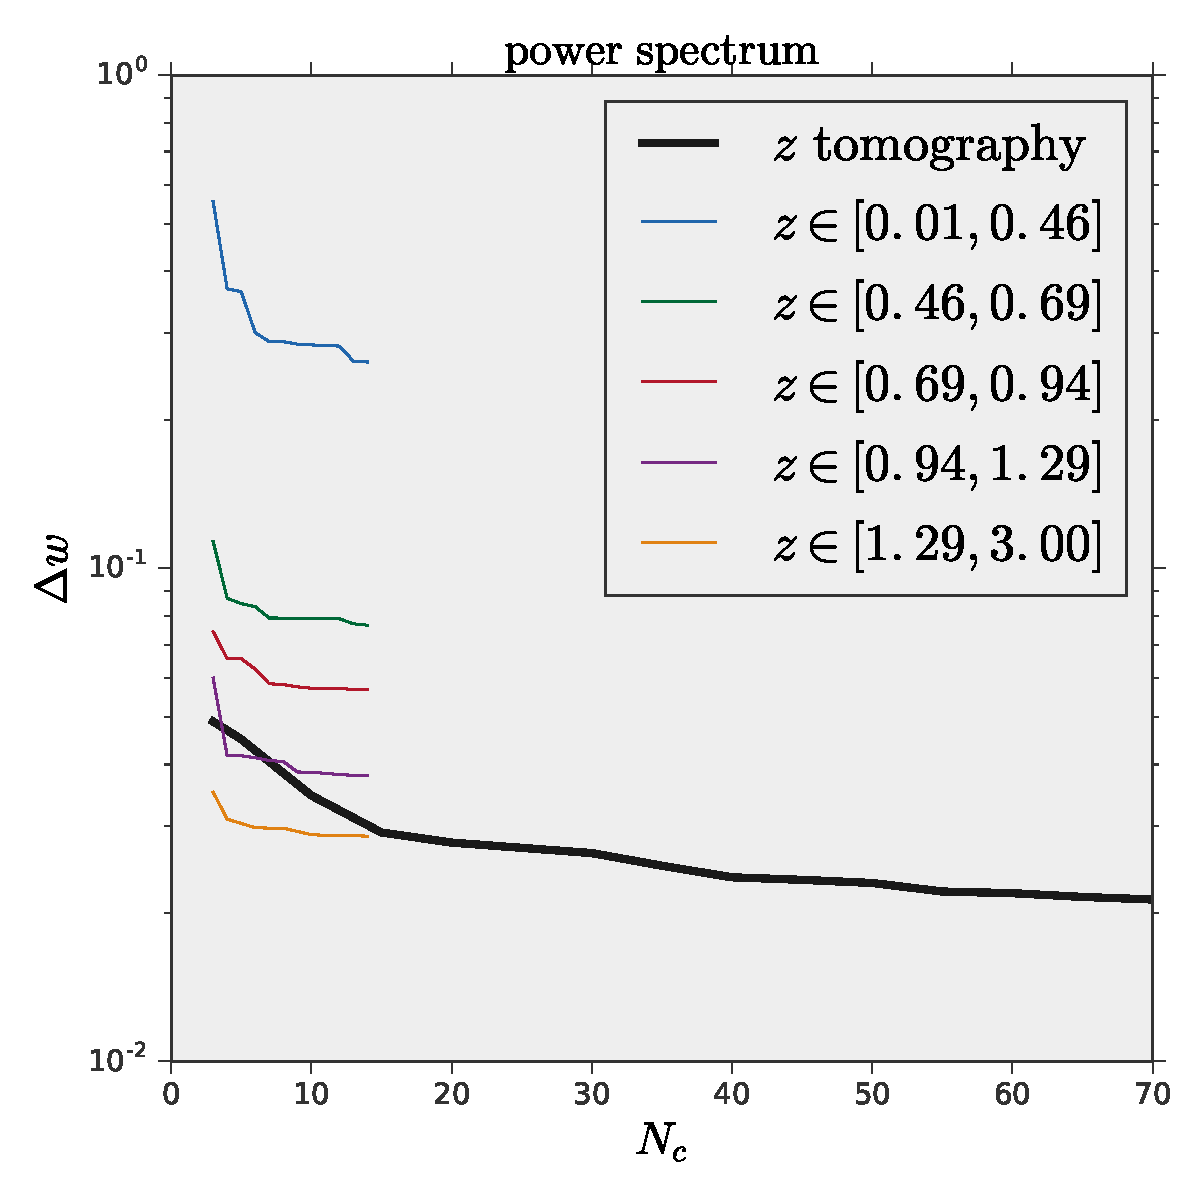
\includegraphics[scale=0.3]{Figures/w_power_spectrum_pca.eps}
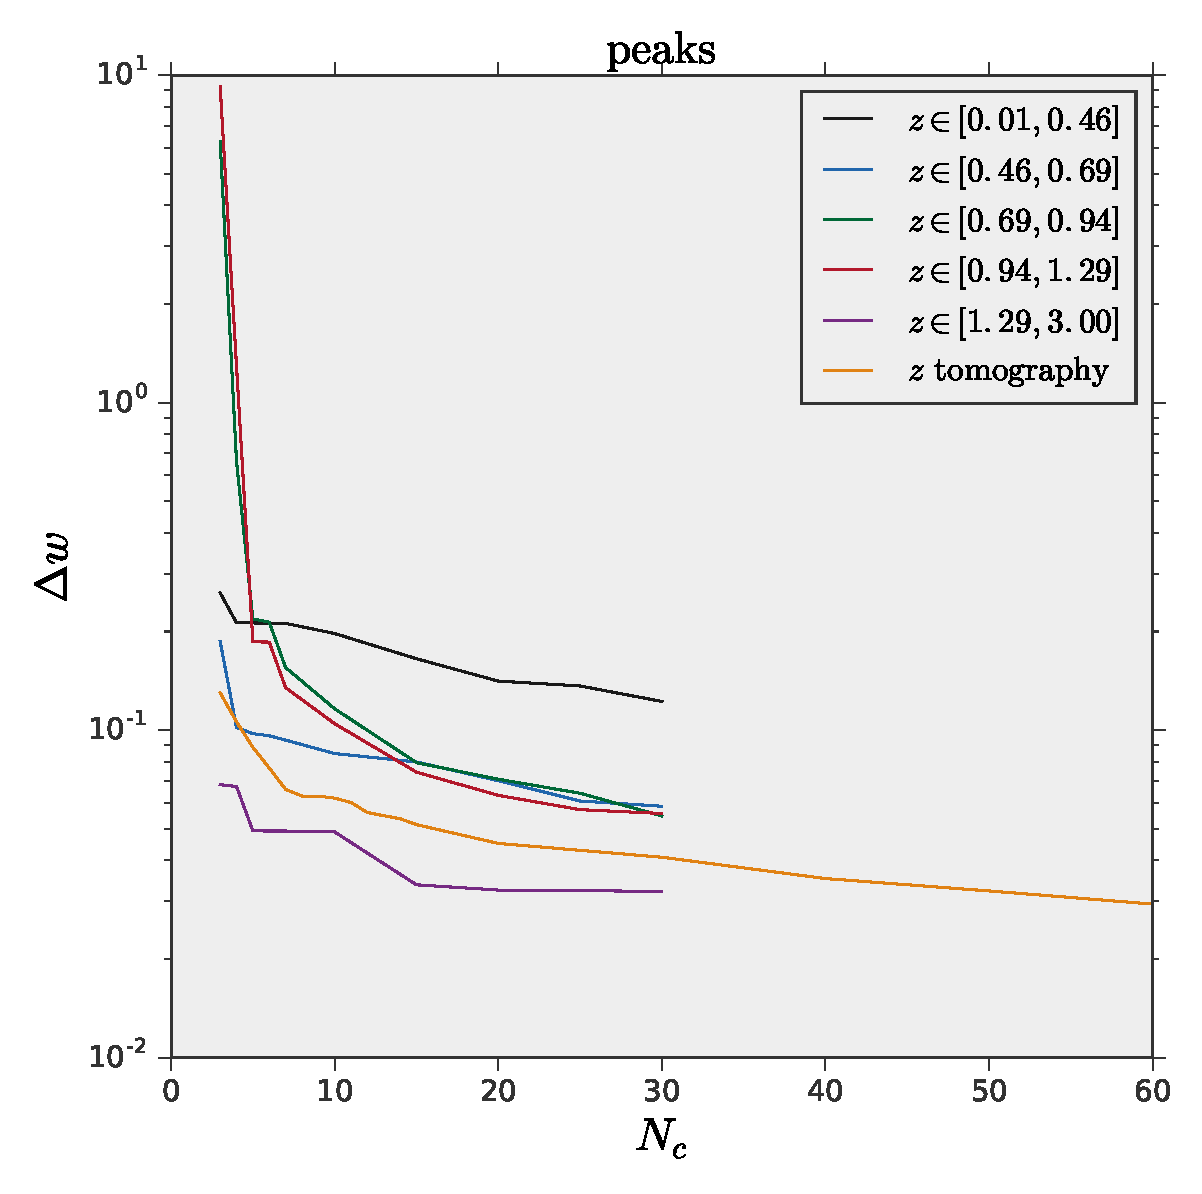
\includegraphics[scale=0.3]{Figures/w_peaks_pca.eps}
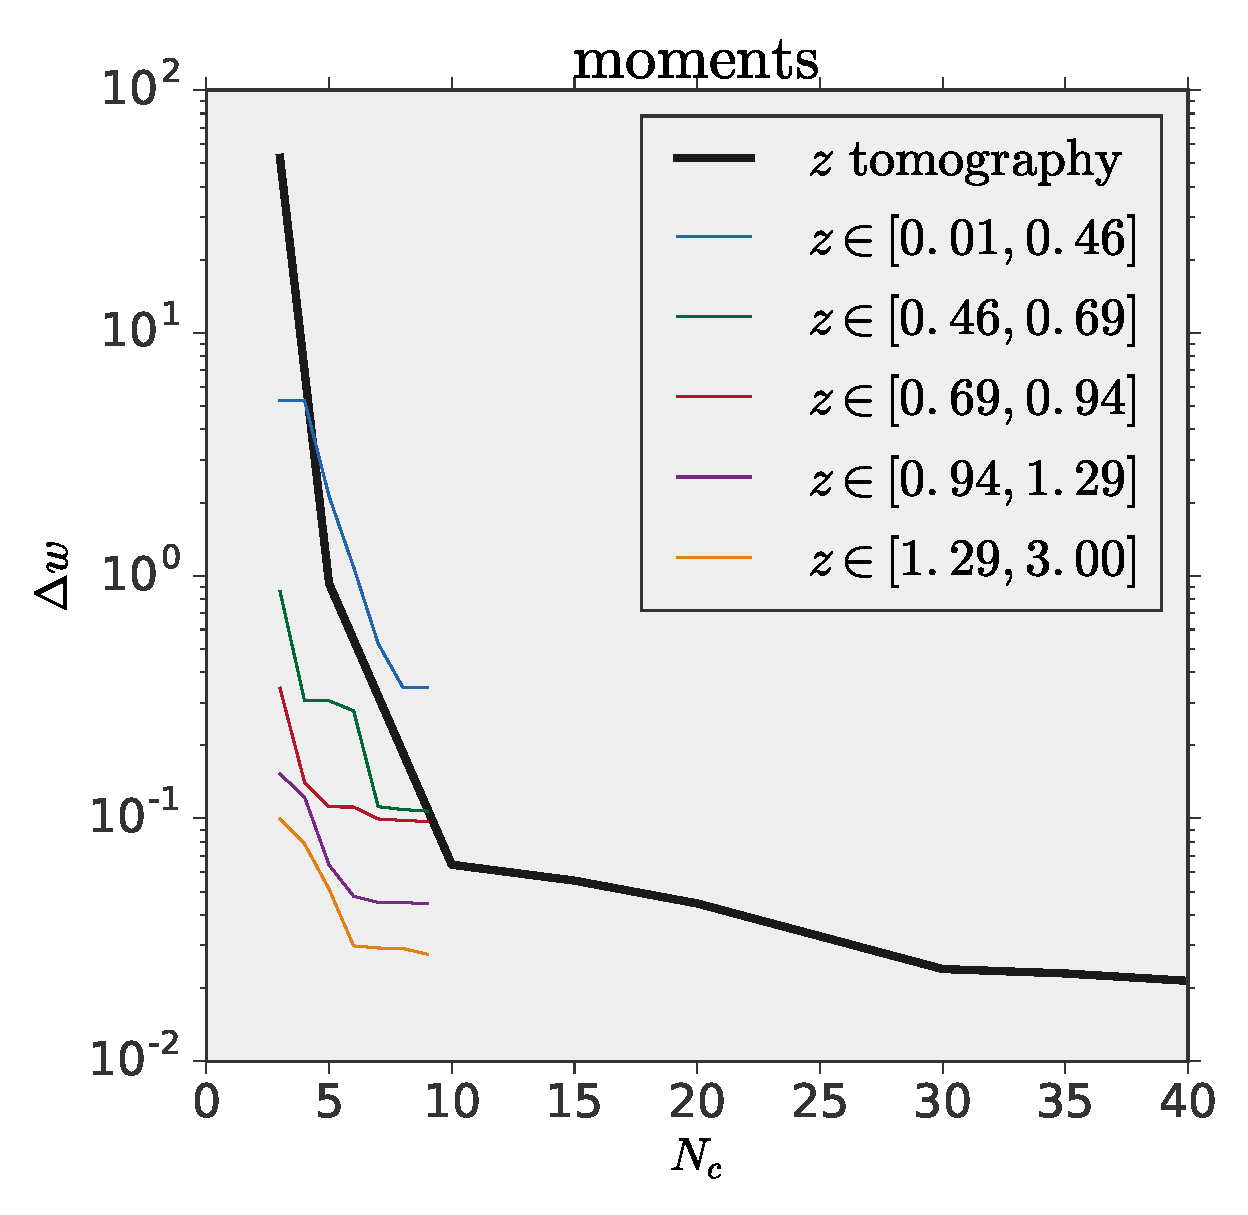
\includegraphics[scale=0.3]{Figures/w_moments_pca.eps}
\caption{$1\sigma$ errors on $w$, marginalized over $(\Omega_m,\sigma_8)$, as a function of the number of the principal components $N_c$, using the power spectrum (top left), peak counts (top right) and moments (bottom). The thin colored lines refer to single redshift summary statistics, while the thick black line shows the case in which the joint redshift information is included.}
\label{fig:pcacomponents}
\end{figure*}

In this section we illustrate the main results of this work. Figure \ref{fig:pcacomponents} shows the robustness of the dimensionality reduction technique we adopted. on the three summary statistics considered, namely the convergence power spectrum $P^{\kappa\kappa}(\ell,\bar{z}_b,\bar{z}_{b'})$, peak counts $n_{\rm pk}(\nu,\bar{z}_b)$ and moments $\pmb{\mu}(\bar{z}_b)$. To measure the power spectrum we chose 15 uniformly spaced multipole bands between $(\ell_{\rm min},\ell_{\rm max})=(200,2000)$. Because, of the combinations $(\bar{z}_b,\bar{z}_{b'})$, only 15 of them (5 diagonal + 10 off-diagonal) are independent, this leads to a total of $N_b=15\times 15=225$ power spectrum measurement bands, including cross redshift information. 
We bin the convergence peak counts in 30 uniformly spaced $\nu$ bins between $(\nu_{\rm min},\nu_{\rm max})=(-2,7)$, for a total of $N_b=30\times5=150$ measurement bands, including redshift information. The total size of the moments summary statistic vector is $N_b=9\times 5=45$, including redshift information. 

The forecast error bars on $w$ are calculated according to equation (\ref{meth:parcovestimator}), where the covariance matrix $\bbh{C}$ and its inverse $\bbh{\Psi}$ have been estimated with $N_r=16000$ realizations of each summary statistic in the fiducial cosmology.

Figure \ref{fig:nopca} shows a comparison between the $w$ constraints obtained using single redshift bins, with and without PCA dimensionality reduction, and compares these single redshift constraints with the ones obtained using redshift tomography. 

\begin{figure*}
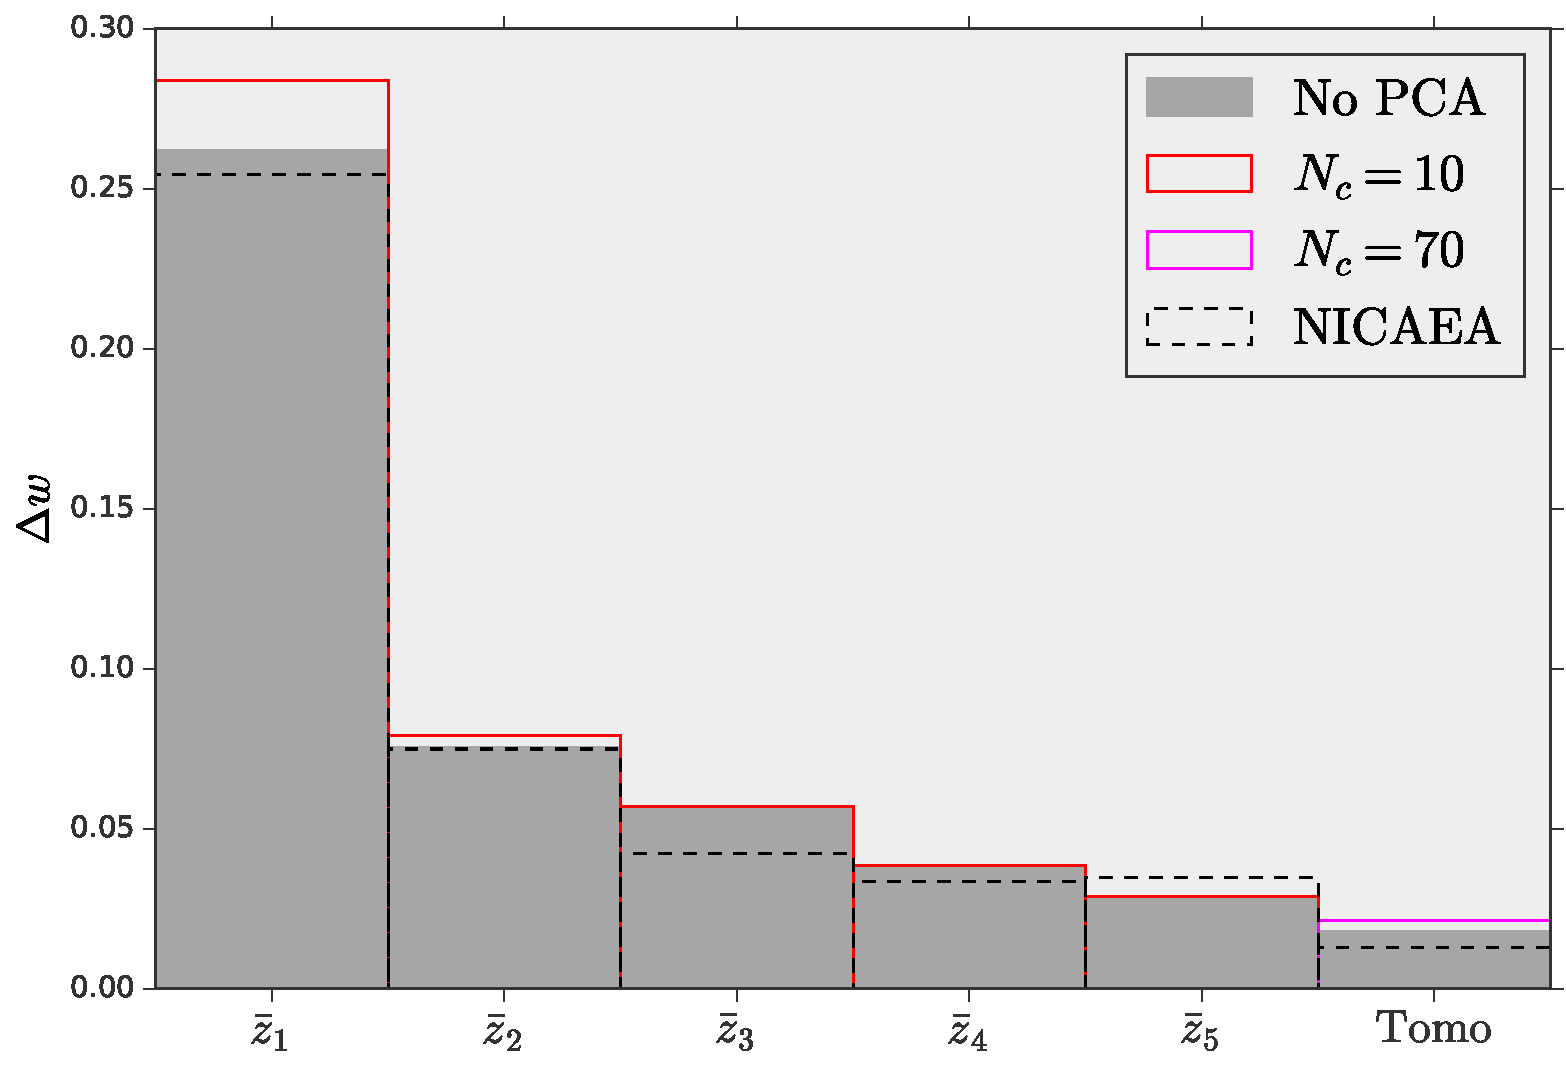
\includegraphics[scale=0.3]{Figures/w_power_spectrum_no_pca.pdf}
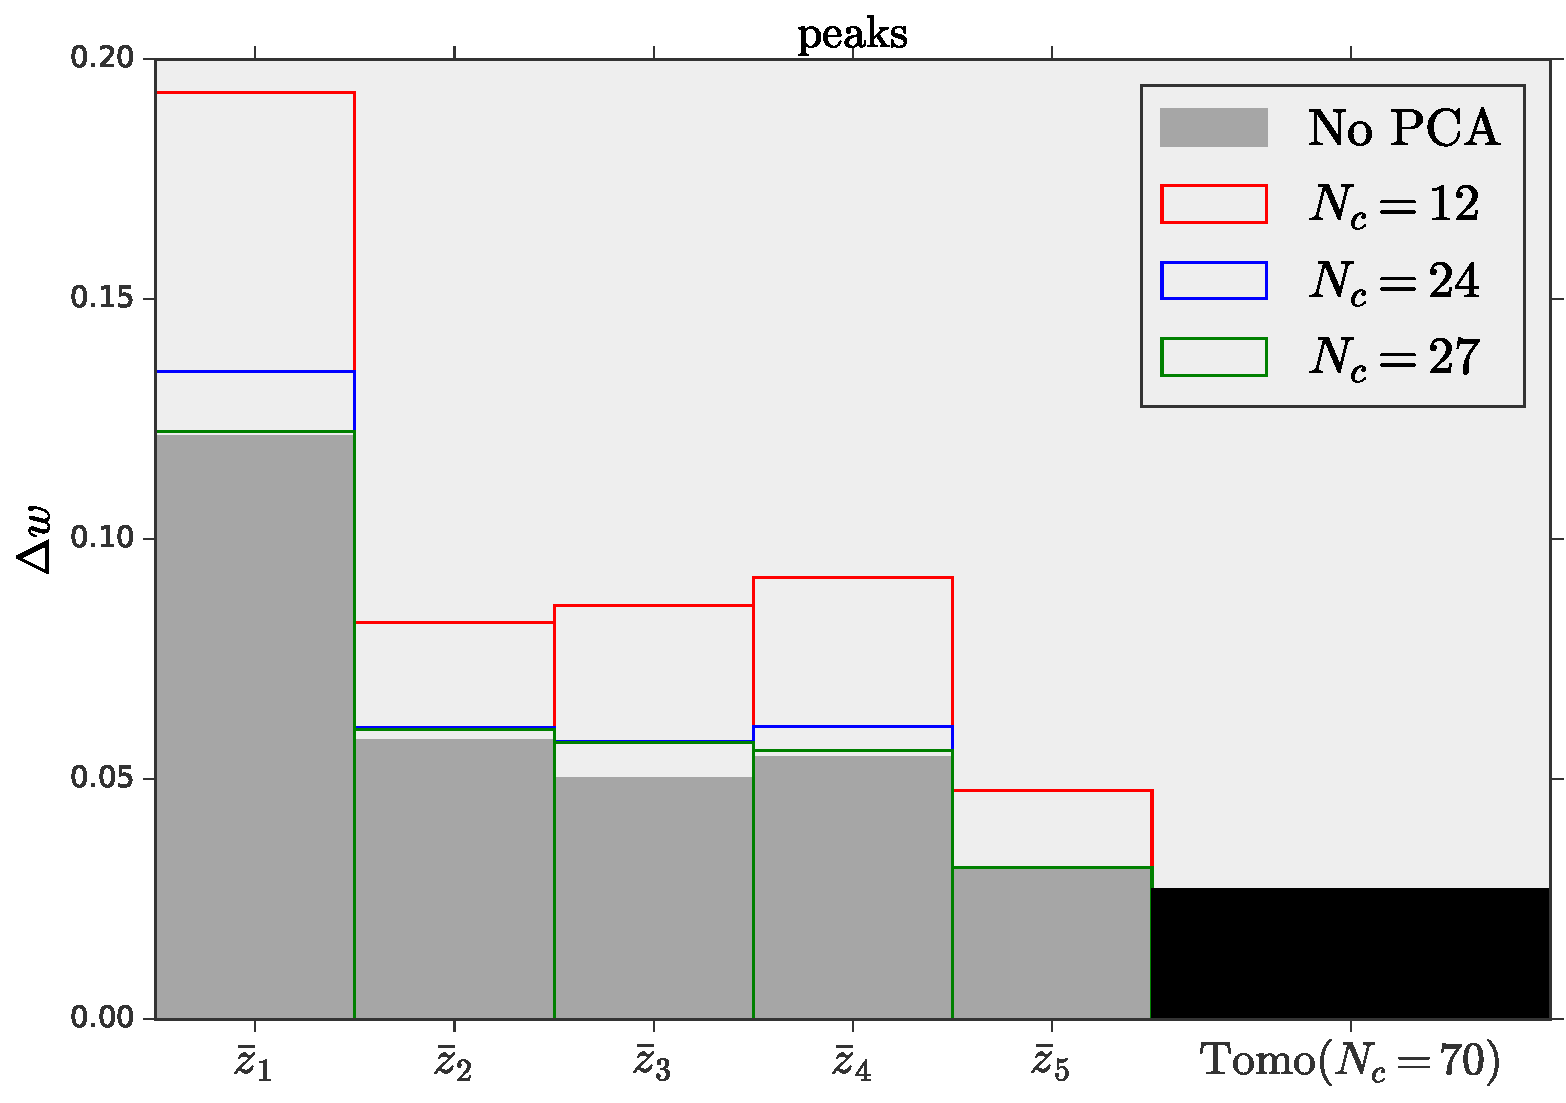
\includegraphics[scale=0.3]{Figures/w_peaks_no_pca.pdf}
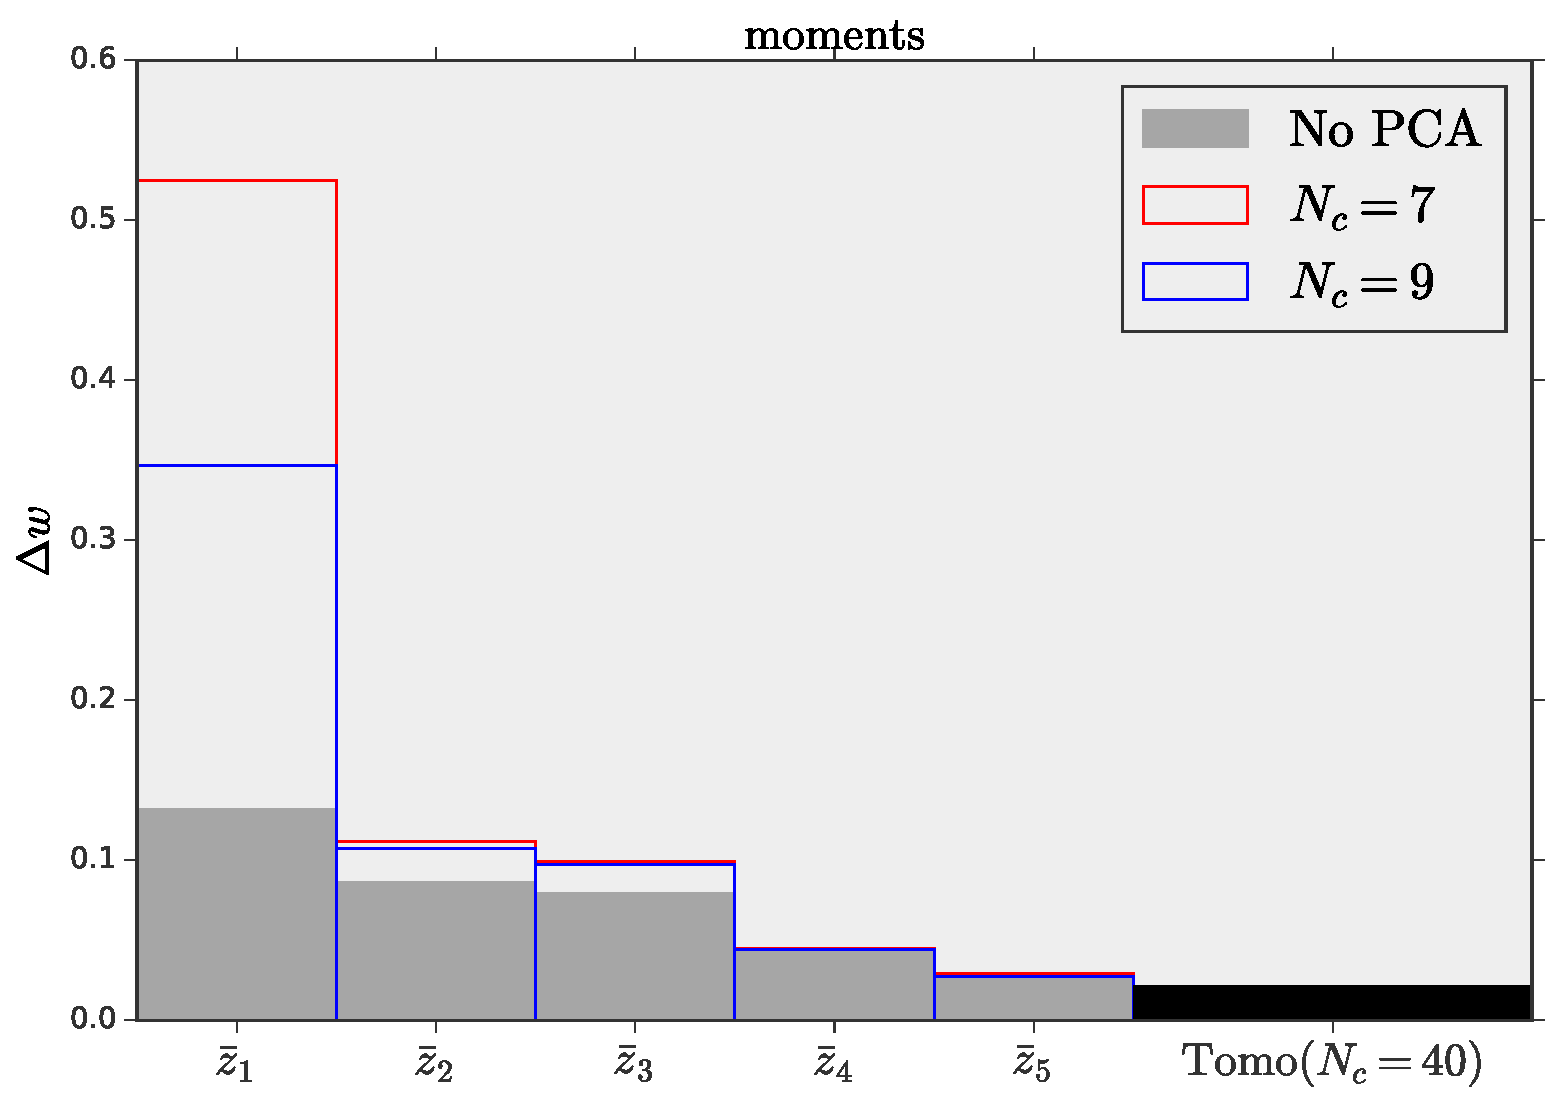
\includegraphics[scale=0.3]{Figures/w_moments_no_pca.pdf}
\caption{Comparison between single redshift $w$ constraints (marginalized over $(\Omega_m,\sigma_8)$) obtained without PCA (gray shaded bars) and with PCA (colored bars) as a function of the redshift bin $\bar{z}_b$. The rightmost black bar shows the same constraint, but obtained with redshift tomography and using the maximum number of PCA components seen in Figure \ref{fig:pcacomponents}. We show constrained obtained with the power spectrum (top right), peak counts (top left) and moments (bottom).}
\label{fig:nopca}
\end{figure*}

Figure \ref{fig:constraintsOm-w} shows the $1\sigma$ confidence contours on the $(\Omega_m,w)$ doublet calculated with equation (\ref{meth:parcovestimator}) after the PCA dimensionality reduction performed according to equation (\ref{meth:pcaprojection}), for a variety of choices $({\rm statistic},N_c)$. We also show the improvements on the confidence contours when combining different summary statistics after the corresponding dimensionality reductions have been performed. 

Figure \ref{fig:photozbias} shows the effect of ignoring photo-$z$ errors on parameter constraints. To evaluate this effect we construct different mock observations, with and without photo-$z$ effects, and compare the results of the parameter fit according to equation (\ref{meth:parestimate}). Using our simulation suite, we construct 20 mock observations: the summary statistic in each observation is calculated by taking the mean of a random sample of $N_{\rm FOV}$ realizations of the summary statistic in the fiducial cosmology (randomly chosen among the ensemble of $N_r=16000$ that are available in the ensemble). The estimated covariance matrix $\bbh{C}$ is scaled by a factor $N_{\rm FOV}$ to take into account the construction process of the mock observations. This procedure allows to forecast the results an LSST-like survey would obtain.        

\begin{figure}
\includegraphics[scale=0.3]{Figures/constraints_Om-w.eps}
\caption{$1\sigma$ confidence contours on the $(\Omega_m,w)$ parameter space, marginalized over $\sigma_8$, obtained using equation (\ref{meth:parcovestimator}). The covariance matrix $\bbh{C}$ and its inverse $\bbh{\Psi}$ have been obtained using $16000$ summary statistics realizations, and has been scaled by a factor $N_{\rm FOV}=1600$ to mimic the constraining power of an LSST-like survey.}
\label{fig:constraintsOm-w}
\end{figure}

\begin{figure}
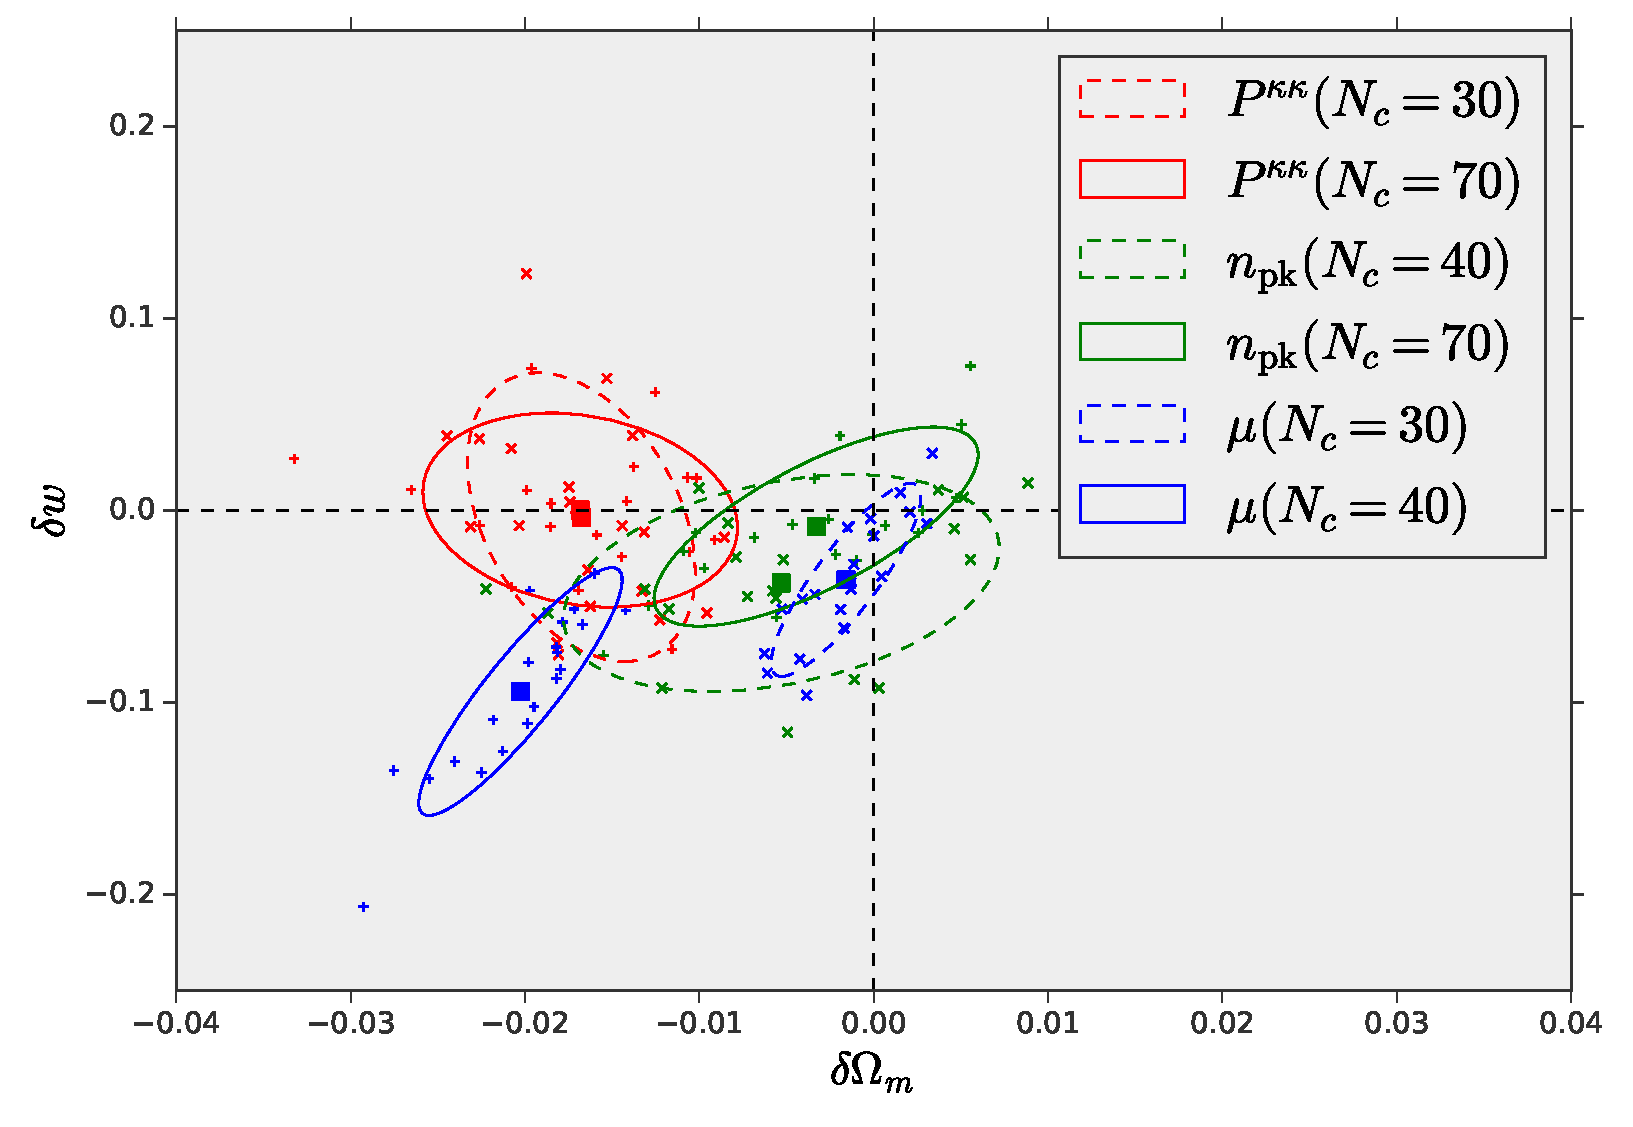
\includegraphics[scale=0.3]{Figures/photoz_bias_Om-w.eps}
\caption{Distribution of parameter estimates in the $(\Omega_m,w)$ parameter space using the power spectrum (red), peak counts (green) and moments (blue) to fit 20 LSST-like mock observations. The parameter deviations $(\delta\Omega_m,\delta w)$ are obtained comparing parameter estimates according to equation (\ref{meth:parestimate}) with and without photo-$z$ errors. The colored squares and the ellipses correspond to respectively to the mean and $1\sigma$ level of the $(\delta\Omega_m,\delta w)$ distribution in the pessimistic systematics case, assuming this distribution is Gaussian.}
\label{fig:photozbias}
\end{figure}

%%%%%%%%%%%%%%%%%%%%%%% DISCUSSION %%%%%%%%%%%%%%%%%%%%%%%%%%%%%%%%%%%%%%%%%%%%%%%%%%%%%%%

\section{Discussion}
In this section we discuss our findings. Figure \ref{fig:pcacomponents} shows that our dimensionality reduction technique is robust. For all the summary statistics we consider, we notice that a plateau in the $w$ error is reached for a sufficient high number of principal components $N_c$. We also see that for single redshift statistics, this plateau is reached for $\sim 5$ components for the power spectrum and the moments, and $\sim 10$ components for the peak counts. Moreover, Figure \ref{fig:nopca} shows that, at least for the four highest redshift bins $\{\bar{z}_b: b\geq 2\}$, most of the cosmological information contained in the full (pre-PCA) summary statistic vector can be captured with a limited number of principal components $N_c<N_b$.   

The number of components to consider increases when including redshift information, and can reach $\sim 30$ for the power spectrum and moments and $\sim 40$ for the peak counts. Figure \ref{fig:nopca} clearly that most of the cosmological information is concentrated in the last redshift bin. The use of redshift tomography only tightens the constraints by a few $10\%$.  

In Figure \ref{fig:constraintsOm-w} we can see that peak counts and moments can significantly improve the constraints on $(\Omega_m,w)$ when combined with the power spectrum. Combining the peaks or the moments to the power spectrum improves the $w$ constraint by a factor of 1.7 while considering the three statistics together the error improves by an additional $30\%$. This shows that peaks and moments contain cosmological information that is not contained in the power spectrum, because a similar improvement cannot be obtained by simply increasing the number of PCA components in the power spectrum dimensionality reduction procedure. 

Figure \ref{fig:photozbias} quantifies the effect of uncorrected photo-$z$ errors on $(\Omega_m,w)$ constraints. Because the random nature of the observations, parameter values $\bbh{p}$ estimated from equation (\ref{meth:parestimate}) are affected by statistical fluctuations. In Figure \ref{fig:photozbias} we show 20 random draws from the probability distribution of $\delta \bbh{p}=\bbh{p}_{\rm photo-z}-\bbh{p}_{\rm no-photo-z}$. We can conclude that the $\bbh{p}$ estimator is biased if $\langle\delta\bbh{p}\rangle\neq 0$. Figure \ref{fig:photozbias} clearly show that photo-$z$ errors cause parameter biases at more than $1\sigma$ significance level when using the power spectrum and the moments, while no bias is observed for the peak count statistic within the constraining accuracy. We also observe that photo-$z$ errors bias the constraints in different directions, leaving open possibilities for bias self--calibration techniques.         

%%%%%%%%%%%%%%%%%%%%%%% CONCLUSIONS %%%%%%%%%%%%%%%%%%%%%%%%%%%%%%%%%%%%%%%%%%%%%%%%%%%%%%%

\section{Conclusions}
In this work we study cosmological parameter constraints forecasts for an LSST-like galaxy survey using the convergence power spectrum and a range of non--Gaussian statistics. We make use of redshift tomography to improve the constraints from their single redshift counterparts. We also investigate the effects of uncorrected photo-$z$ systematic effects on the inferred cosmology. We find that:
\begin{itemize}
	\item Principal Component analysis is a robust technique to keep the dimensionality of the parameter space under control and avoid the numerical pitfalls explained in \citep{Taylor12,DodelsonSchneider13,Taylor14} and more recently \citep{PetriVariance}. In particular we find that only a few components are necessary to characterize the cosmological information content in single redshift statistics, while more components are necessary when tomography is included. Nevertheless we find that the number of required components $N_c$ is significantly smaller than the full summary statistic space dimensionality before performing PCA.
	\item Most of the cosmological information is contained in high redshift galaxies, with tomography improving $w$ constraints by only a few $10\%$.   
	\item Peak counts and moments can significantly improve $(\Omega_m,w)$ parameter constraints when used in combination with the power spectrum.
	\item Uncorrected photo-$z$ systematics can bias parameter constraints obtained from the power spectrum and the moments, but in different parameter directions, leaving open windows for self-calibration
\end{itemize}

%%%%%%%%%%%%%%%%%%%%%%%%%% ACKNOWLEDGMENTS %%%%%%%%%%%%%%%%%%%%%%%%%%%%%%%%%%%%%%%%%%%%%%

\section*{Acknowledgments}

%%%%%%%%%%%%%%%%%%%%%%%%%%%%%%%%%%%%%%%%%%%%%%%%%%%%%%%%%%%%%%%%%%%%%%%%%%%%%%%%%%%%%%%%%%

\bibliography{ref}

\label{lastpage}
\end{document}
